\documentclass[13pt]{article}
\usepackage{amsmath, amsthm, amssymb, graphicx, enumitem, esvect}


% Language setting
% Replace `english' with e.g. `spanish' to change the document language
\usepackage[english]{babel}

% Set page size and margins
% Replace `letterpaper' with `a4paper' for UK/EU standard size
\usepackage[letterpaper,top=2cm,bottom=2cm,left=3cm,right=3cm,marginparwidth=1.75cm]{geometry}

\title{C\&EE 110 Homework 2}
\author{Warren Kim}

\begin{document}
\maketitle

\newpage
\section*{Problem 1}
The conditional probabilities of the different failure mechanisms
given a hazardous event are given below:
\begin{itemize}
\item $P(S|E_S) = 0.3$
\item $P(S|E_M) = 0.03$
\item $P(F|V_H) = 0.1$
\item $P(F|V_M) = 0.02$
\item $P(F|V_L) = 0.005$
\item $P(S|V_H) = P(S|V_M) = P(S|V_L) = P(F|E_S) = P(F|E_M) = 0$
\item $P(E_S) = 0.10$
\item $P(E_M) = 0.90$
\item $P(V_H) = 0.08$
\item $P(V_M) = 0.22$
\item $P(V_L) = 0.7$
\end{itemize}
Additionally, the probability of occurrence for a strong or mild
earthquake is $0.10$ and $0.90$ respectively. The probability of
occurrence for a high, medium, or low vertical load odue to the trucks
is $0.08$, $0.22$, and $0.7$ respectively. Please answer:

\begin{enumerate}[label=\textbf{\alph*.}]
\item What does the expression
  \[P(S|V_H) = P(S|V_M) = P(S|V_L) = P(F|E_S) = P(F|E_M) = 0\]
  mean in practice? For the answer, relate the failure mechanism to
  the different hazardous event.

\item Determine the probability that an earthquake causes a shear
  failure.

\item Determine the probability that the traffic of the trucks causes
  a flexure failure.

\item Let's suppose that a flexure failure occurs, what is the
  probability that the traffic load was medium?

\item Now let's suppose that a shear failure occurs, what is the
  probability that the earthquake was strong?
\end{enumerate}

\subsection*{Response}
\begin{enumerate}[label=\textbf{\alph*.}]
\item A shear failure can never happen due to vertical load and a
  flexure failure can never happen due to an earthquake.
\item
  \begin{align*}
    P(S|E) &= P(S|E_S)P(E_S) + P(S|E_M)P(E_M) \\
           &= (0.3)(0.1) + (0.03)(0.9) \\
           &= 0.03 + 0.027 \\
    P(S|E) &= 0.057
  \end{align*}

\item
  \begin{align*}
    P(F|V) &= P(F|V_H)P(V_H) + P(F|V_M)P(V_M) + P(F|V_L)P(V_L) \\
           &= (0.1)(0.08) + (0.02)(0.22) + (0.005)(0.7) \\
           &= 0.008 + 0.0044 + 0.0035 \\
    P(F|V) &= 0.0159
  \end{align*}

\item 
  \begin{align*}
    P(V_M|F) &= \frac{P(F|V_M)P(V_M)}{P(F)} \\
             &= \frac{(0.02)(0.22)}{0.0159} \\
             &= \frac{0.0044}{0.0159} \\
    P(V_M|F) &= 0.277
  \end{align*}
  
\item
  \begin{align*}
    P(E_S|S) &= \frac{P(S|E_S)P(E_S)}{P(S)} \\
             &= \frac{(0.3)(0.1)}{0.057} \\
             &= \frac{0.03}{0.057} \\
    P(E_S|S) &= 0.526
  \end{align*}
\end{enumerate}





\newpage
\section*{Question 2}
Relays used in construction of electric circuits function properly if
current can flow through them when the circuit is closed.
\begin{enumerate}[label=\textbf{\alph*.}]
\item Asuming that the circuits are independent, which fo the
  following ciruit designs yields a higher probability that the
  current will flow when the relays are activated?
  \begin{center}
    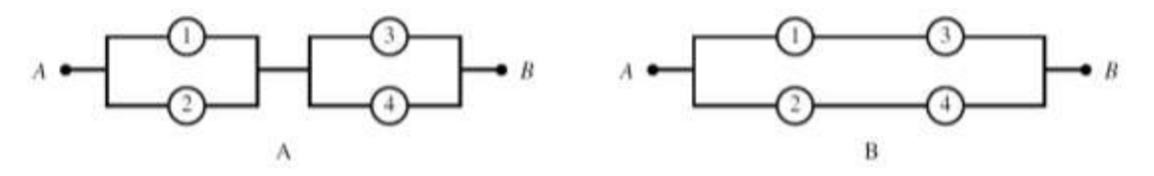
\includegraphics[scale=0.25]{images/circuits.png}
  \end{center}

\item If we know that the relay elements 1 and 2 are dependent as
  $P(F_1|F_2) = 0.03)$. How does this change the answer?
\end{enumerate}
The probability of failure of each element is:
\begin{center}
  \begin{tabular}{|l|l|}
    \hline
    \textbf{Relay Element} & \textbf{Proability of Failure (F)} \\
    \hline
    1 & 0.13 \\ \hline
    2 & 0.02 \\ \hline
    3 & 0.10 \\ \hline
    4 & 0.30 \\
    \hline
  \end{tabular}
\end{center}

\subsection*{Response}
\begin{enumerate}[label=\textbf{\alph*.}]
\item
  \begin{align*}
    P(F_A) &= P(F_1 \cap F_2) \cup P(F_3 \cap F_4) \\
           &= P(F_1)P(F_2) + P(F_3)P(F_4) - P(F_1)P(F_2)P(F_3)P(F_4) \\
           &= (0.13)(0.02) + (0.10)(0.30) - (0.13)(0.02)(0.10)(0.30) \\
           &= 0.0026 + 0.03 - 0.0000078 \\
    P(F_A) &= 0.0327 \implies P(S_A) = 0.967 \\ \\
    P(S_B) &= P(S_1 \cap S_3) \cup P(S_2 \cap S_4) \\
           &= P(S_1)P(S_3) + P(S_2)P(S_4)  - P(S_1 \cap S_2 \cap S_3 \cap S_4) \\
           &= P(S_1)(P(S_3) + P(S_2)P(S_4)  - P(S_1)P(S_2)P(S_3)P(S_4) \\
           &= (0.87)(0.90) + (0.98)(0.70) - (0.87)(0.98)(0.90)(0.70) \\
    P(S_B) &= 0.932
  \end{align*}
  Circuit $A$ is more reliable.

\item
  \begin{align*}
    P(F_A) &= P(F_1 \cap F_2) \cup P(F_3 \cap F_4) \\
           &= P(F_1|F_2)P(F_2) + P(F_3)P(F_4) - P(F_1|F_2)P(F_2)P(F_3)P(F_4) \\
           &= (0.03)(0.02) + (0.10)(0.30) - (0.03)(0.02)(0.10)(0.30) \\
           &= 0.0006 + 0.03 - 0.000018 \\
    P(F_A) &= 0.0306 \implies P(S_A) = 0.969 \\ \\
    P(F_B) &= P(F_1 \cup F_3) \cap P(F_2 \cup F_4) \\
           &= [P(F_1) + P(F_3) - P(F_1)P(F_3)][P(F_2) + P(F_4) - P(F_2)P(F_4)] \\
           &= [0.13 + 0.10 - (0.13)(0.10)][0.02 + 0.30 - (0.02)(0.30)] \\
    P(F_B) &= 0.0681 \implies P(S_B) = 0.932
  \end{align*}
  Circuit $A$ is more reliable.
\end{enumerate}





\newpage
\section*{Question 3}
\begin{itemize}
\item $P(X) = 0.6$
\item $P(Y) = 0.3$
\item $P(Z) = 0.1$
\item $P(R|X) = 0.5$
\item $P(R|Y) = 0.6$
\item $P(R|Z) = 0.9$
\end{itemize}
Suppose that we randomly select one coolant tank in the manufacturer's
factory. What is the probability that this tank:
\begin{enumerate}[label=\textbf{\alph*.}]
\item is created from recycled materials?
\item is produced in company $Y$ from recycled materials?
\item is produced in company $Y$, given that the tank is craeted from
  recycled materials?
\item is created from recycled materials, given that it is produced by
  company $Z$?
\end{enumerate}

\subsection*{Response}
\begin{enumerate}[label=\textbf{\alph*.}]
\item
  \begin{align*}
    P(R) &= P(R|X)P(X) + P(R|Y)P(Y) + P(R|Z)P(Z) \\
         &= (0.5)(0.6) + (0.6)(0.3) + (0.1)(0.9) \\
         &= 0.3 + 0.18 + 0.09 \\
    P(R) &= 0.57
  \end{align*}

\item
  \begin{align*}
    P(R \cap Y) &= P(R|Y)P(Y) \\
                &= (0.6)(0.3) \\
    P(R \cap Y) &= 0.18
  \end{align*}

\item
  \begin{align*}
    P(Y|R) &= \frac{P(R|Y)P(Y)}{P(R)} \\
           &= \frac{(0.6)(0.3)}{0.57} \\
           &= \frac{0.18}{0.57} \\
    P(Y|R) &= 0.316
  \end{align*}

\item
  \begin{align*}
    P(R|Z) &= 0.9
  \end{align*}
\end{enumerate}





\newpage
\section*{Question 4}
Concrete can experience three different types of defects. Let $A_i (i
= 1, 2, 3)$ denote the event that the concrete has a defect of type
$i$. Suppose that
\[P(A_1) = 0.12, \hspace{1em} P(A_2) = 0.07, \hspace{1em} P(A_3) =
  0.05\]
\[P(A_1 \cup A_2) = 0.13, \hspace{1em} P(A_1 \cup A_3) = 0.14,
  \hspace{1em} P(A_2 \cup A_3) = 0.10\]
\[P(A_1 \cap A_2 \cap A_3) = 0.01\]
\begin{enumerate}[label=\textbf{\alph*.}]
\item What is the probability that the concrete does not have a type 1
  defect?
\item What is the probability that the concrete has both type 1 and
  type 2 defects?
\item What is the probability that the concrete has both type 1 and
  type 2 defects but not a type 3 defect?
\item What is the probability that the concrete has at most two of
  these defects?
\end{enumerate}

\subsection*{Response}
\begin{enumerate}[label=\textbf{\alph*.}]
\item $P(\overline{A}_1) = 1 - P(A_1) = 1 - 0.12 = 0.88$

\item
  \begin{align*}
    P(A_1 \cap A_2) &= P(A_1) + P(A_2) - P(A_1 \cup A_2) \\
                    &= 0.12 + 0.07 - 0.13 \\
    P(A_1 \cap A_2) &= 0.06
  \end{align*}

\item
  \begin{align*}
    P(A_1 \cap A_2 \cap \overline{A}_3) &= P(A_1 \cap A_2) - P(A_1
                                          \cap A_2 \cap A_3) \\
                    &= 0.06 - 0.01 \\
    P(A_1 \cap A_2 \cap \overline{A}_3) &= 0.05
  \end{align*}

\item $1 - P(A_1 \cap A_2 \cap A_3) = 1 - 0.01 = 0.99$
\end{enumerate}
\end{document}

%%% Local Variables:
%%% mode: latex
%%% TeX-master: t
%%% End:
